\section{Embedding the even-qubit family}
\label{embed:section}

The unified construction and the earlier even-qubit family provide two phase directions through the same reference measurement. We now ask whether both directions can be varied independently while preserving the tetrahedral geometry. To compare them at the level of the complete measurement, first express the earlier family in the notation of Sec.~\ref{core:framework}. For even $n$, retain
$E_n=\{2,4,\ldots,n-2\}$ and define
\begin{equation}
 q_A(z)=\prod_{j\in E_n}(1-z_j),\qquad d_A(z)=q_A(z)-\delta_{z,0}.
 \label{embed:and-support}
\end{equation}
The diagonal $i^{f_0(z)}e^{i\alpha d_A(z)}$ is precisely the even-qubit family of Pauwels and Gisin~\cite{PauwelsGisin2026}, with $\alpha=\pi\tau/2$ in their parameter convention. Its background depends only on the even internal coordinates. Every character $h$ in Table~\ref{core:pullback-table} contains a coordinate outside $E_n$, so a flip of that coordinate cancels the background expectation. Moreover, $q_A(a)=1$ for class I and $q_A(a)=0$ for class II. Equation~\eqref{core:signal} then gives the common signed component $c_n\cos\alpha$, and hence $r=r_E(n)\cos\alpha$ for $|\alpha|\le\pi/2$. This argument includes $n=2$, where the product is empty and $q_A=1$, and $n=4$, where $q_A=1-z_2$.

For even $n\ge8$, this family and the unified enhanced family are coordinate sections of a two-parameter family. Write $d_B=d_n$ for the support in Eq.~\eqref{core:support} and set
\begin{align}
 D_{\alpha,\beta}(z)&=i^{f_0(z)}e^{i\alpha d_A(z)+i\beta d_B(z)},\notag\\
 M_n(\alpha,\beta)&=C_nD_{\alpha,\beta}H^{\otimes n}.
 \label{embed:measurement}
\end{align}
Figure~\ref{fig:embedding} shows the two-parameter family and its coordinate sections.
\begin{figure*}[tbp]
  \centering
  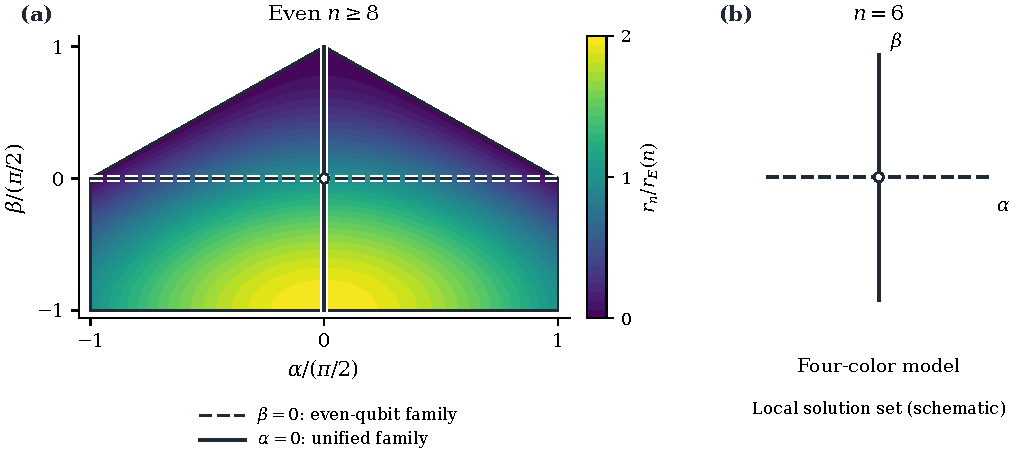
\includegraphics[width=\textwidth]{figures/fig2_embedding.pdf}
  \caption{Two exact sections of an even-qubit two-parameter family.
  (a) For even $n\geq8$, the domain $\Omega$ is given by $|\alpha|\leq\pi/2$ and $-\pi/2\leq\beta\leq\pi/2-|\alpha|$.
  Color represents $r_n/r_E(n)=\cos\alpha-\sin\beta$, with reference radius $r_E(n)=\sqrt3/2^{n-1}$; both axes are in units of $\pi/2$.
  The dashed section $\beta=0$ recovers the prior even-qubit cosine family, and the solid section $\alpha=0$ recovers the unified enhanced family, in each case column by column.
  The open circle marks the common base point.
  (b) Schematic local solution set at $n=6$ in the four-color model, with phases assigned to the four values of $(q_A,q_B)$ and an independent zero-string phase: the two branches cross at the base point.}
  \label{fig:embedding}
\end{figure*}

\begin{theorem}[Two-parameter embedding]
\label{embed:theorem}
For every even $n\ge8$, Eq.~\eqref{embed:measurement} defines an orthonormal measurement for all real $\alpha,\beta$. All its signed seed components equal
\begin{equation}
 m_n(\alpha,\beta)=c_n(\cos\alpha-\sin\beta).
 \label{embed:component}
\end{equation}
On the domain
\begin{equation}
 \Omega=\left\{(\alpha,\beta): |\alpha|\le\frac\pi2,\quad
 -\frac\pi2\le\beta\le\frac\pi2-|\alpha|\right\},
 \label{embed:domain}
\end{equation}
the measurement has the fixed local tetrahedra of Eq.~\eqref{core:bloch-orbit}, with
\begin{align}
 r_n(\alpha,\beta)&=r_E(n)(\cos\alpha-\sin\beta),\notag\\
 r_n(\Omega)&=[0,2r_E(n)].
 \label{embed:radius}
\end{align}
Its $\beta=0$ section recovers the earlier even-qubit family column by column, and its $\alpha=0$ section recovers Theorem~\ref{core:unified-theorem} column by column. The two parameter directions are independent as ordered measurement projectors.
\end{theorem}

The essential step is cancellation of the joint background. Put $u=e^{i\alpha}$ and $v=e^{i\beta}$. The seed before applying $-iC_n$ is
\begin{equation}
 2^{-n/2}\left[\sum_z i^{|z|}u^{q_A(z)}v^{q_B(z)}\ket z
 +(i-uv)\ket{0^n}\right],
 \label{embed:seed}
\end{equation}
where $q_B=q_n$. At every class-I flip, $(q_A(a),q_B(a))=(1,0)$; at every class-II flip, the pair is $(0,1)$. Their defect contributions therefore agree, because
\begin{align}
 \operatorname{Re}[-iu^{-1}(i-uv)]
 &=\cos\alpha-\sin\beta,\notag\\
 \operatorname{Re}[-v^{-1}(i-uv)]
 &=\cos\alpha-\sin\beta.
 \label{embed:defect}
\end{align}
Class I leaves $q_A$ unchanged, reducing its background to the already vanishing $q_B$ background. In class II, the AND difference separates the background sum into the three sectors $q_A(z)-q_A(z\oplus a)=1,0,-1$. In the first sector all even internal bits vanish. For $n\ge8$, there are at least two odd internal bits, and any nonconstant character on this block cancels by a parity-preserving pair flip. Only six fixed four-bit sums remain; their coefficients vanish exactly. Appendix~\ref{embed:appendix} supplies the full classification and the six finite identities. This establishes Eq.~\eqref{embed:component} for every even $n\ge8$, after which the orbit formula gives all reduced states.

On $\Omega$, $\sin\beta\le\cos\alpha$, while $\cos\alpha-\sin\beta\le2$; the $\alpha=0$ section attains every value between zero and two. The two axis identities follow directly from the diagonal entries in Eq.~\eqref{embed:measurement}. To check that the parameters survive passage to projectors, note that a diagonal infinitesimal input phase $A$ produces only column phases exactly when $AH^{\otimes n}=H^{\otimes n}B$ for a diagonal $B$. Every Hadamard entry is nonzero, so $A$ and $B$ must be the same scalar. The pairs $(d_A,d_B)$ take the values $(0,0),(1,0),(0,1)$ at $0,e_1,e_1\oplus e_2$, respectively. No nonzero linear combination of the two directions is scalar.

\begin{proposition}[Crossing branches at $n=6$]
\label{embed:six-proposition}
For $n=6$, the direct superposition in Eq.~\eqref{embed:measurement} has equal signed components if and only if $\sin\alpha\sin\beta=0$. More generally, assign independent phases to the four values of $(q_A,q_B)$ and an independent phase to the physical zero string. Near the specified EJM, the regular measurements in this model consist exactly of the two original one-parameter branches.
\end{proposition}
Here the odd internal block contains only one bit. The $X_3$ and $X_4$ background expectations acquire the additional normalized term $-\sin\alpha\sin\beta/8$, while the other components retain their common defect value. The local equations of this four-color phase model are solved in Appendix~\ref{embed:appendix}. Thus the enhanced family exists at $n=6$, but this particular two-parameter extension reduces locally to a crossing of its two axes.
